\documentclass{article}
\usepackage[english]{babel}
\usepackage[utf8x]{inputenc}
\usepackage[T1]{fontenc}
\usepackage[space]{xeCJK}
\usepackage[fontset=ubuntu]{ctex}
\usepackage{graphicx} 
\usepackage{listings}
\usepackage{booktabs}

\usepackage{geometry}   %设置页边距的宏包
\usepackage{titlesec}   %设置页眉页脚的宏包
\usepackage{color}

\definecolor{dkgreen}{rgb}{0,0.6,0}
\definecolor{gray}{rgb}{0.5,0.5,0.5}
\definecolor{mauve}{rgb}{0.58,0,0.82}

\lstset{ %
  language=Octave,                % the language of the code
  basicstyle=\footnotesize,           % the size of the fonts that are used for the code
  numbers=left,                   % where to put the line-numbers
  numberstyle=\tiny\color{gray},  % the style that is used for the line-numbers
  stepnumber=2,                   % the step between two line-numbers. If it's 1, each line 
                                  % will be numbered
  numbersep=5pt,                  % how far the line-numbers are from the code
  backgroundcolor=\color{white},      % choose the background color. You must add \usepackage{color}
  showspaces=false,               % show spaces adding particular underscores
  showstringspaces=false,         % underline spaces within strings
  showtabs=false,                 % show tabs within strings adding particular underscores
  frame=single,                   % adds a frame around the code
  rulecolor=\color{black},        % if not set, the frame-color may be changed on line-breaks within not-black text (e.g. commens (green here))
  tabsize=2,                      % sets default tabsize to 2 spaces
  captionpos=b,                   % sets the caption-position to bottom
  breaklines=true,                % sets automatic line breaking
  breakatwhitespace=false,        % sets if automatic breaks should only happen at whitespace
  title=\lstname,                   % show the filename of files included with \lstinputlisting;
                                  % also try caption instead of title
  keywordstyle=\color{blue},          % keyword style
  commentstyle=\color{dkgreen},       % comment style
  stringstyle=\color{mauve},         % string literal style
  escapeinside={\%*}{*)},            % if you want to add LaTeX within your code
  morekeywords={*,...}               % if you want to add more keywords to the set
}

\geometry{left=3cm,right=2.5cm,top=2.5cm,bottom=2.5cm} 

%% You can change the font if necessary.
% \setCJKmainfont{BabelStone Han}
% \setCJKsansfont{Noto Sans CJK SC}

\title{基于VR简笔画的模型检索 \\ 中期答辩}
\author{
罗宇辰 516030910101 \\
陈志扬 516030910347 \\
陈\quad 诺516030910199
}
\begin{document}


\maketitle
\tableofcontents

\clearpage
\newpage


\section{课程设计题目}
本小组的设计题目是 \textbf{基于VR简笔画的模型检索}。

我们希望能够研发一个通过VR简笔画输入来进行模型检索来获得模型的系统,
并且将这个系统作为一个子模块加入中学生VR实验系统中,
为中学生提供一个更便利的获得模型的交互方式。

\section{项目目标与创新简述}
\subsection{项目目标}
我们希望能够研发一个VR交互友好、模型检索高效准确的系统。

通过这个系统,我们希望能够改善学生在VR中做实验的交互方式,并且降低实验设计者的工作量。 
\subsection{创新简述}
创新点主要有两部分:
\begin{enumerate}
    \item 将VR信息作为输入的基于内容的模型检索
    \item VR下的交互与特征提取
\end{enumerate}

\subsubsection{以VR信息为输入的基于内容的模型检索}
常见的模型检索方法分为基于语义的检索和基于内容的检索。 

基于语义的检索显然不适合VR下的交互,因为VR中大多数操作都以Touch, Grab来完成,
所以在VR环境下输入文字是一件很费时费力的事情。 

而基于内容的交互中比较传统的方法是基于图片的搜索。例如百度就推出了百度搜图的功能。
在VR环境下,得到承载检索信息载体的\textbf{内容}确实一件不太容易的事情——让用户在VR中挑图片未免太不方便。
因此我们想直接使用VR中用户能很方便使用Touch, Grab等操作的特点,直接让用户在VR环境下使用较少的步骤画出简笔画作为检索需要的信息。

\subsubsection{VR下的交互与特征提取}
由于交互方式为VR,因此我们需要实现VR下的交互与特征提取。

处于直接在三维中绘图会有出界、不同视图会变得奇怪的问题,我们选择在VR中为用户提供一个黑板来作为交互方式
。用户通过Touch来在VR环境下绘制二维图像。VR端再将包含有用户输入信息的图像发送给模型检索端。

模型检索端获得用户输入后,需要先预处理用户的输入,再将处理过的图片传递给特征提取模块。

\section{HCI思想}
\begin{enumerate}
    \item 贴近用户习惯
    
    \qquad 从用户的角度出发,考虑方便性:开题时考虑到在三维空间中画三维图更方便,于是设定了 画三维图像→特征提取→转化为二维图像→匹配识别 的流程。但是在实际的实践中,我们发现了一些问题。
    
    \qquad 对于普通的中学生和老师,在未经训练的情况下,更习惯于在二维平面作画,也就是所谓的纸笔作画。三维空间中的凭空绘制虽然也并不难以学习,但是其稳定程度、作画的舒适感相对来说有些不符合人体工程学。
    
    \qquad 我们发现黑板这样一个在三维空间中提供作画平台的工具在中学教室里非常常见,几乎每个人都有机会接触,也有过接触经验。在课程中我们讲到过人的记忆仓库会对一些长期存在的记忆有偏好,一些长期记忆会渐渐规则化、潜意识化。我们人机界面的设计原则中很重要的一点就是要减少学习适应的信息总量,使用用户更为熟悉的固有记忆。我们发现黑板作画放在我们的VR环境中会非常容易接受。

    \item 按键位置
    
    设计在黑板右侧,符合大多数人的习惯。
    
    \item 图标
    
    图标图案选取是大家比较熟悉且易懂的标识符
    
\end{enumerate}

\clearpage

\section{设计思路与技术}

系统整体架构如图一所示,主要分为两个模块:VR模块和模型检索模块。

\begin{figure}[htb]
\centering
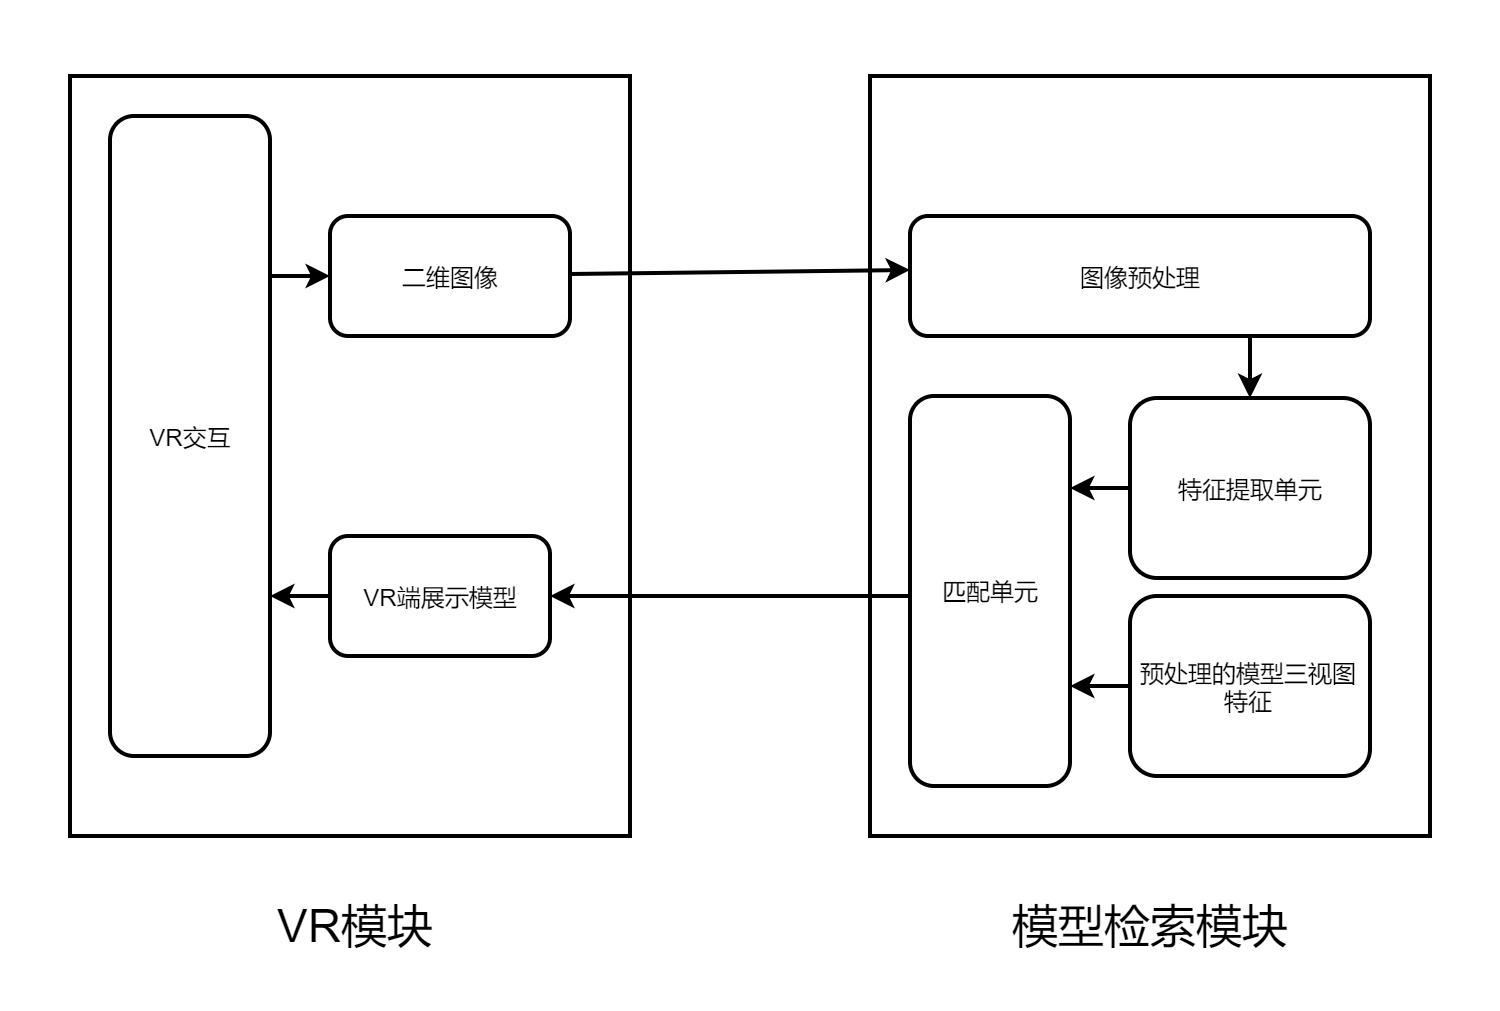
\includegraphics[width=1\textwidth]{images/architecture.png}
\caption{系统架构}\label{fig:digit}
\end{figure} 

\subsection{设计思路}

\subsubsection{VR模块}
设计考虑与调整:

在开题报告中我们考虑到,用户在三维空间中更方便进行三维的绘图,于是决定使用tilt brush在unity中进行开发。但在实践阶段遇到了两个问题:
\begin{enumerate}
    \item tilt brush整合
    
    \qquad google tilt brush 的相关教程较少。google tilt brush更多是一个开发好了的绘图工具,与unity整合在一起获取画出的模型资源有难度。
    
    \item 三维绘图的误差
    
    \qquad 我们在开题阶段就注意到,三维模型的绘制会出现从不同视角看过去差别较大的情况。考虑到大部分未经过训练的用户更习惯于普通的在画纸上进行二维创作的习惯,在实践中也会习惯在三维空间里画二维图像(也就是物体的主视图)。而此时二维图像的线段容易不在一个平面内,考虑过的多视图加权计算思路操作起来并不容易。
    
\end{enumerate}

 \qquad 综合以上考虑,为了在中期能够收获一个实验结果,在VR端的设计上做出了改动:在空间中固定一个画板,为用户提供一个可参考的二维平面,然后提供画笔让用户进行绘画。

\subsubsection{模型检索模块}
模型检索模块分为如下几个部分:
\begin{itemize}
    \item 图像预处理模块
    \item 特征提取模块
    \item 预处理的模型三视图特征模块
    \item 匹配单元模块
\end{itemize}

\begin{enumerate}
    \item 图像预处理模块

\qquad 图像预处理主要是将VR端输入的信息进行二次处理。

\qquad 用户在操作时很可能会将多余的信息引入图片中,例如不小心点上的点、断断续续的线、歪歪扭扭的直线等。
为了降低此类因素给特征提取单元的带来的误差,所以我们在VR输入和特征提取单元之间加入了图片预处理模块。
    
    
    \item 特征提取模块
    
\qquad 特征提取模块主要目的是提取出VR输入信息中的特征。

\qquad 此模块可以复用从模型三视图中提取特征模块的工程代码。主要目的是找出VR端输入信息中的特征,
并以此为基础来匹配出和输入特征重合度较高的模型。
    
    \item 预处理的模型三视图特征模块

\qquad 预处理模型三视图部分存储了已有模型三视图对应的特征值。

\qquad 通过直接使用预处理的模型三视图特征,能够大大降低模型检索耗费的时间。
    
    \item 匹配模块

\qquad 匹配单元主要通过VR信息提取出的特征值与预处理的模型三视图的特征值来匹配出合适的模型,并返回给VR端。

\end{enumerate}

\clearpage

\subsection{主要技术}

\subsubsection{VR模块}
\begin{enumerate}
    \item 场景设计
    
    \qquad 首先定义了一个黑板(在场景中建一个Quad)和许多画笔。
    
    \begin{figure}[htb]
    \centering
    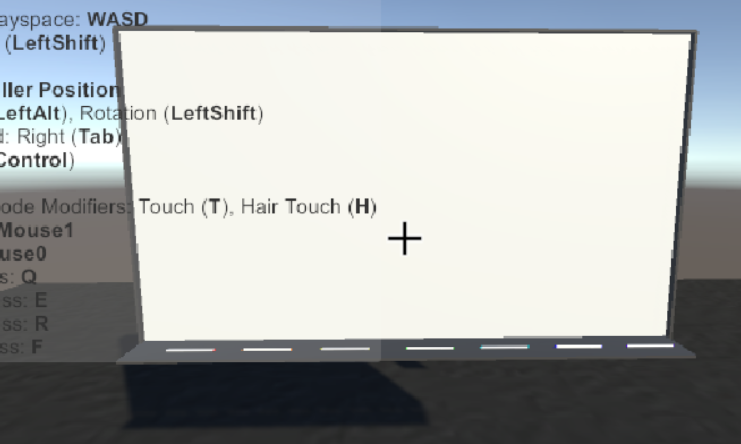
\includegraphics[width=0.8\textwidth]{images/board.png}
    \caption{画板}\label{fig:digit}
    \end{figure} 
    
    
    \qquad 画笔的设计上有些复杂,分为笔的头、尾(控制握笔的方向)还有笔尖(用来绘画)。在画笔触碰到黑板时触发函数记录画笔此刻的位置并将此处的像素点设置颜色,然后实时更新黑板面的texture来显示绘画图案。
    
    \begin{figure}[htb]
    \centering
    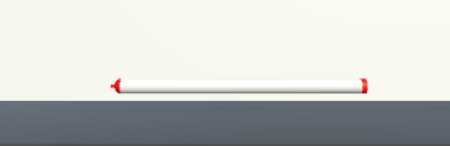
\includegraphics[width=0.8\textwidth]{images/pen.png}
    \caption{画笔}\label{fig:digit}
    \end{figure}
    
    \qquad 在黑板旁边设置两个新的碰撞体,一个用来触发提交功能,将此刻的texture转换成PNG形式保存提交。另一个触发load模型的功能,将检索系统返回的模型信息从模型库中找到并显示在画面中。
    
    \begin{figure}[htb]
    \centering
    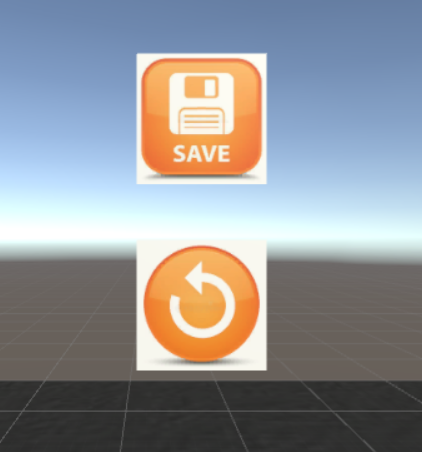
\includegraphics[width=0.6 \textwidth]{images/button.png}
    \caption{两个处理按钮}\label{fig:digit}
    \end{figure}

    \item 功能实现
    
    1. 关于像素点绘制: 
    
    运用Unity Texture2D类中的两个函数:
    
\begin{lstlisting}[title=SetPixel, frame=shadowbox]
public void SetPixels32(int x, int y, int blockWidth, int blockHeight, Color32[] colors, int miplevel = 0);
\end{lstlisting}

    
    
    
    \qquad 前面4个参数相当于一个矩形,x和y就是矩形的左下角的那个点,blockWidth和blockHeight分别是矩形的宽和高,这个矩形所代表的范围就是blockWidth*blockHeight个像素所在的位置,不妨称这个矩形范围为一个色块;
    
    \qquad colors这个参数的大小必须等于blockWidth*blockHeight,因为这个方法就是给坐标(x,y)开始,从左到右,从下到上,一行一行的对矩形范围内的每个像素赋值;也就是把colors[0]~colors[blockWidth - 1]分别赋值到坐标为(x,y)~(x + blockWidth,y)的像素,以此类推;
    
    \begin{lstlisting}[title=Apply, frame=shadowbox]
public void Apply(bool updateMipmaps = true, bool makeNoLongerReadable = false);
\end{lstlisting}
     
     \qquad 当对图片改动完成以后,需要调用这个方法,才能让改动真正的应用在图片上;
    
    \begin{figure}[htb]
    \centering
    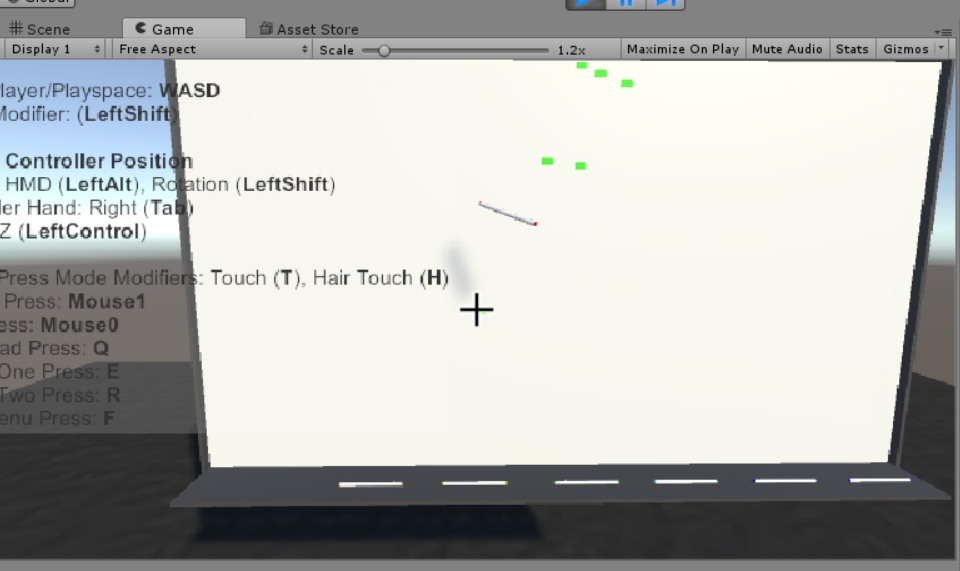
\includegraphics[width=0.7\textwidth]{images/draw.jpg}
    \caption{执笔绘画场景}\label{fig:digit}
    \end{figure} 
    
     
    2.  关于绘画信息传输:
    
    \qquad 当触碰到信息传输的碰撞体时,会将此刻的黑板画面由Texture2D格式转成PNG格式保存下来,用以比对检测。
    
    
    3.  关于模型的展示:
    
    \qquad 当触碰到展示模型的碰撞体时,会在场景中显示prefab库中对应名称(名称信息由检索系统返回)的模型,展示在场景中。
    
\end{enumerate}
 
\clearpage

\subsubsection{模型检索模块}

图片预处理模块的架构如图所示

\begin{figure}[htb]
\centering
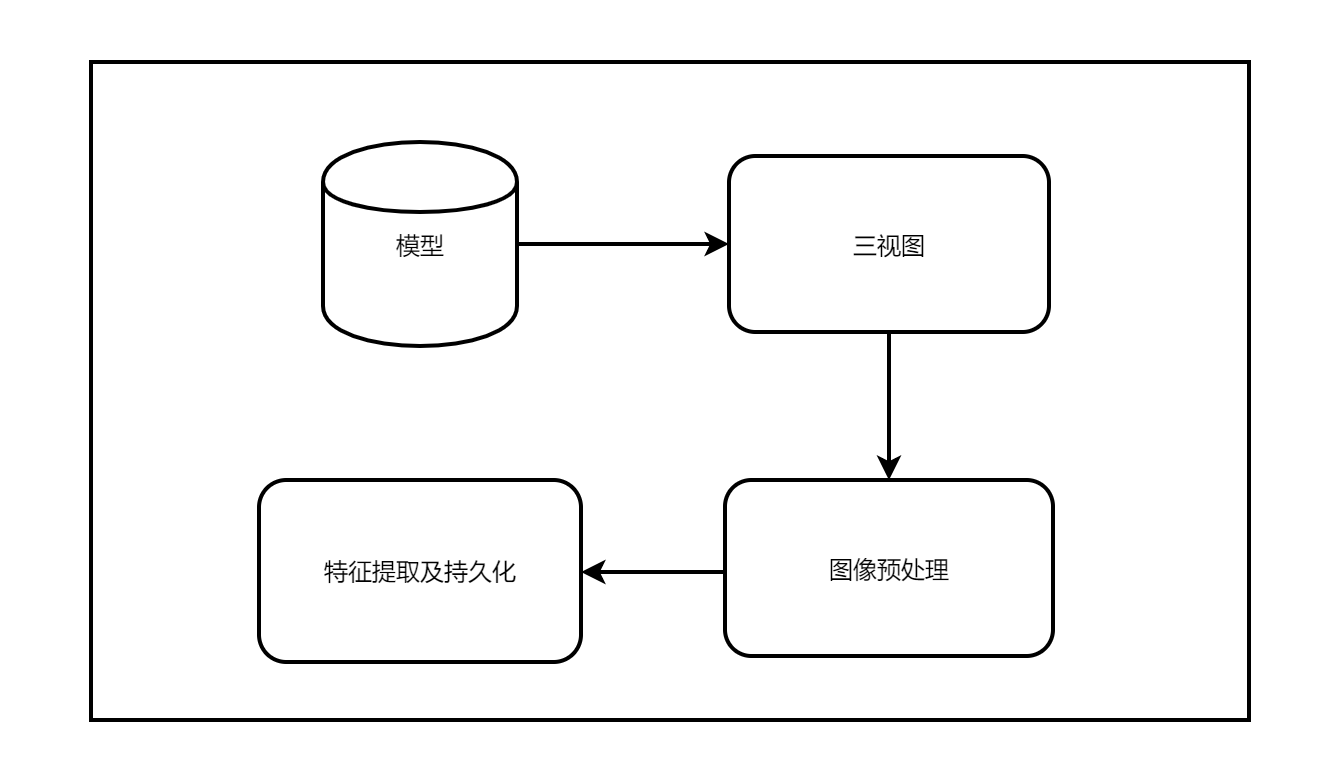
\includegraphics[width=0.8\textwidth]{images/pre-process.png}
\caption{图片预处理模块}\label{fig:digit}
\end{figure} 



\begin{enumerate}
    \item 模型三视图渲染及预处理

我们使用了Blender场景和Python脚本、MATLAB脚本来得到三视图。
    \begin{enumerate}

    \item Blender场景
    
    \begin{figure}[htb]
    \centering
    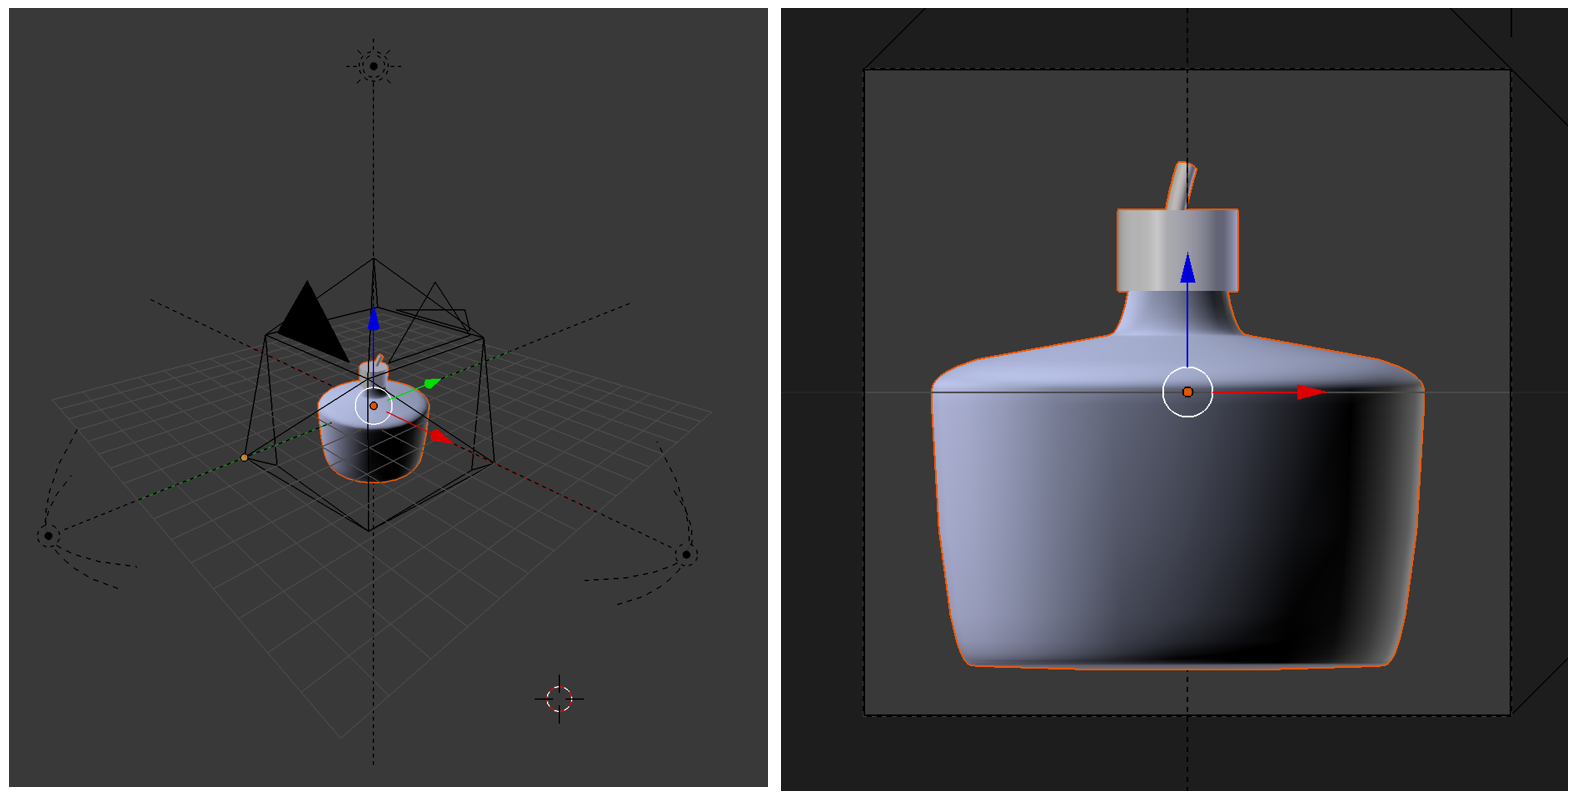
\includegraphics[width=0.8\textwidth]{images/Blender.png}
    \caption{Blender场景}\label{fig:digit}
    \end{figure} 
        
    \qquad 在场景中设置了3个camera,分别拍摄模型的正视图、侧视图和俯视图。
    
    \qquad 由于模型的部分材质是玻璃或者水这样的透明物资,所以我们对模型进行了一些调整,改变了部分Material的高光、透明度、颜色等参数。同时为了渲染出位置、大小合适的图像,对模型的重心和尺寸也进行了调整。


    \item Python脚本
    
    \qquad 使用Python脚本来打开Blender场景文件,load模型,设置渲染并且最终输出三视图图片。
    
    \item MATLAB脚本
    
    \qquad 调用Python脚本对模型进行成批渲染。
    
\begin{figure}[hb]
\centering
\includegraphics[width=1\textwidth]{images/RenderOutput.png}
\caption{渲染结果}\label{fig:digit}
\end{figure} 
    
    \end{enumerate}
    
    
    \item 视图特征提取
    
    \qquad 得到三视图之后,我们期望能够从三视图中提取出模型的特征。
    
    \begin{enumerate}
        \item 提取轮廓特征
        
        \qquad 为了提取出视图特征,首先需要提取出视图中的轮廓图。
        
    \begin{figure}[hb]
    \centering
    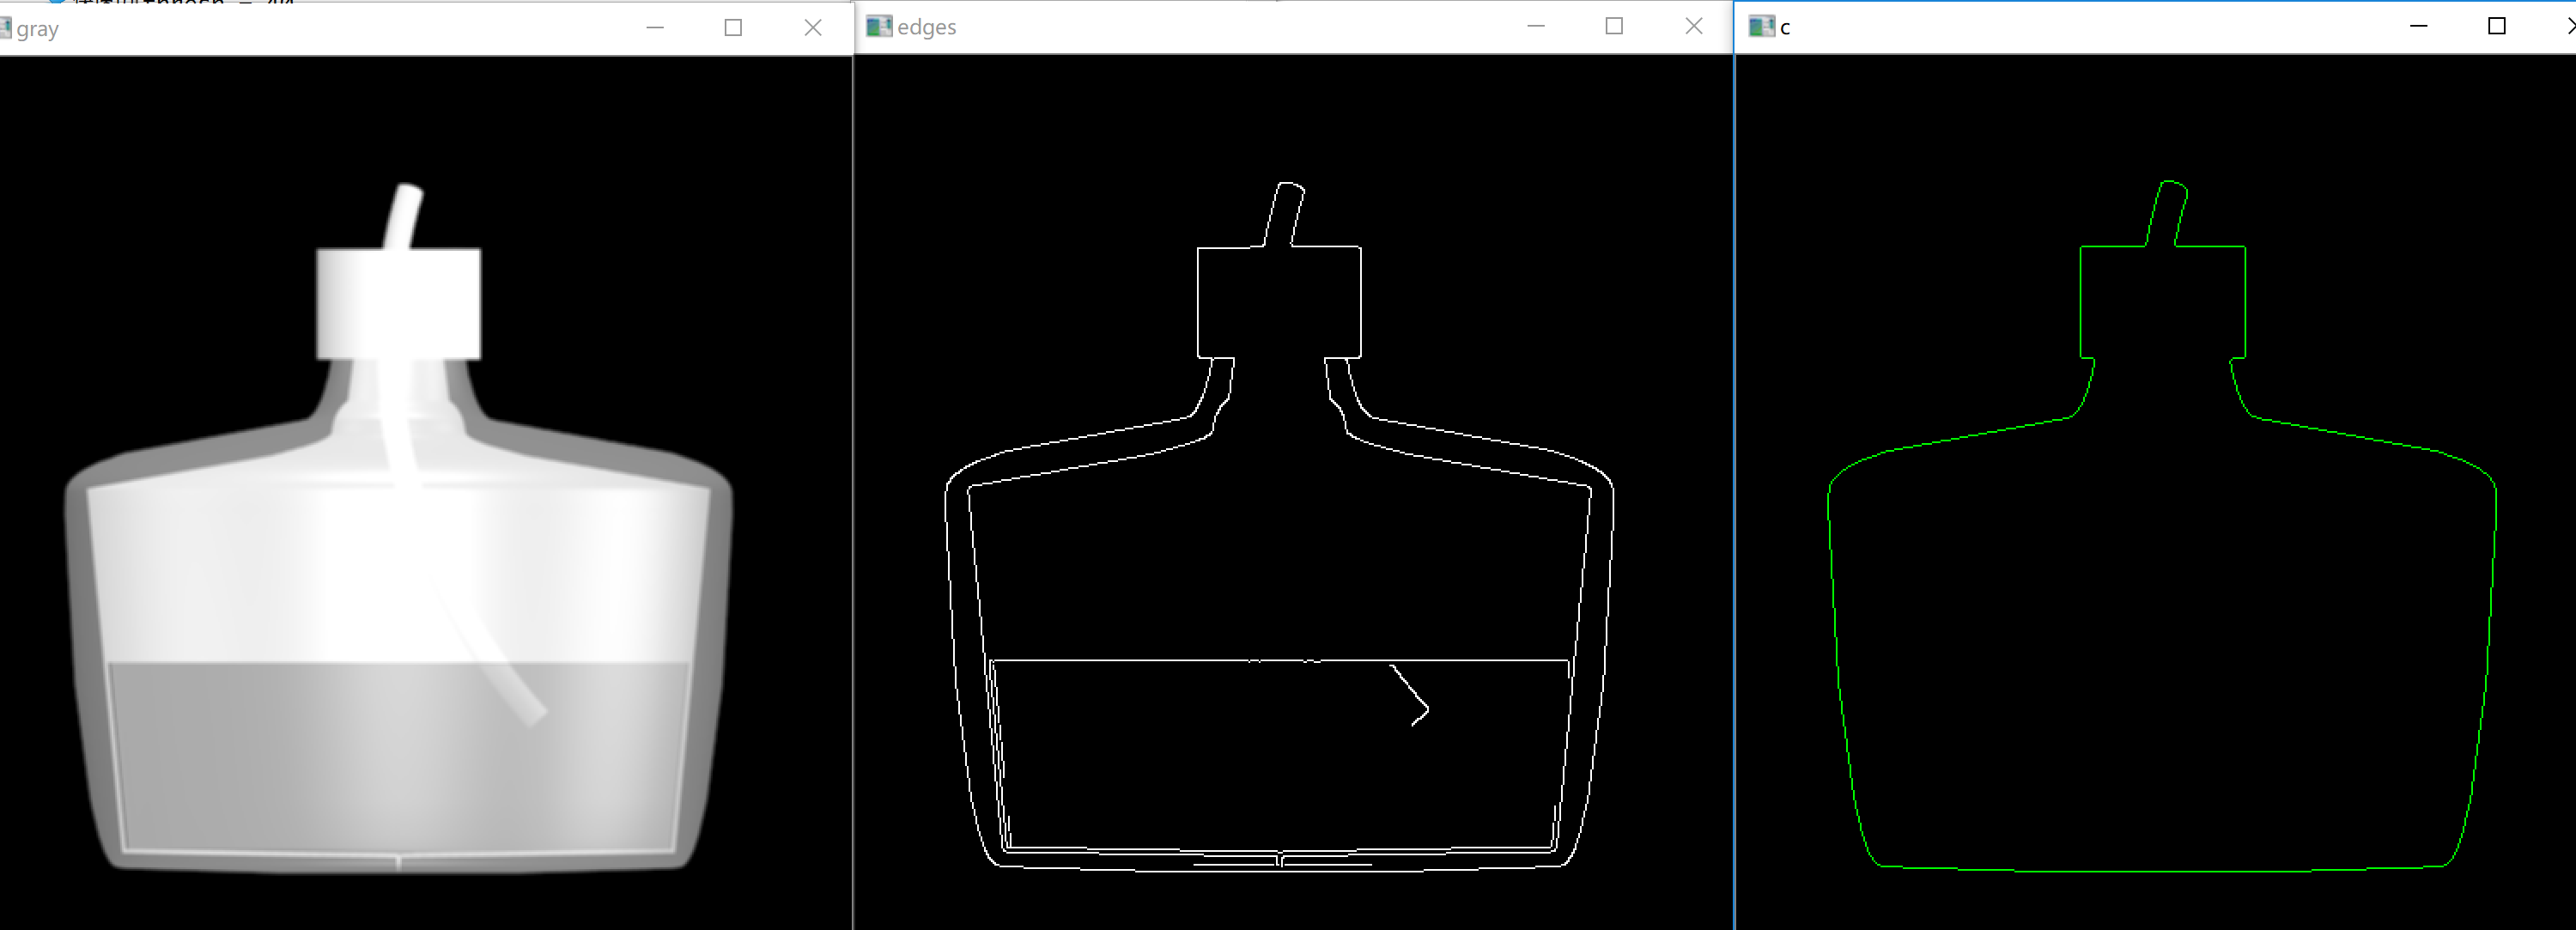
\includegraphics[width=1\textwidth]{images/Canny.png}
    \caption{均值滤波后的灰度图像/Canny边缘检测/外轮廓}\label{fig:digit}
    \end{figure} 
    
    
    \qquad 提取轮廓前首先对图片进行了均值滤波处理。
    
    \qquad Canny能够清晰的识别出图片的内外轮廓。但是使用Canny会有一些局限性:输出结果是二值图像,大小也和原始图像相关。所以使用Canny的话需要对输出结果进行二次处理。
    
    \qquad 最后我们放弃了Canny来提取轮廓,选择了直接使用opencv提供的API: findCountours() 来完成外轮廓的提取(图9最右图),获得了较好的效果。
    
    \item 特征提取
    
    \qquad 图片特征提取中的SIFT (Scale-invariant feature transform) 算子,由于具有尺度不变性、旋转不变性,并且检测效果受图像亮度、拍摄视角音效较小,所以我们首先尝试了SIFT算子提取特征。
    
    \begin{figure}[h]
    \centering
    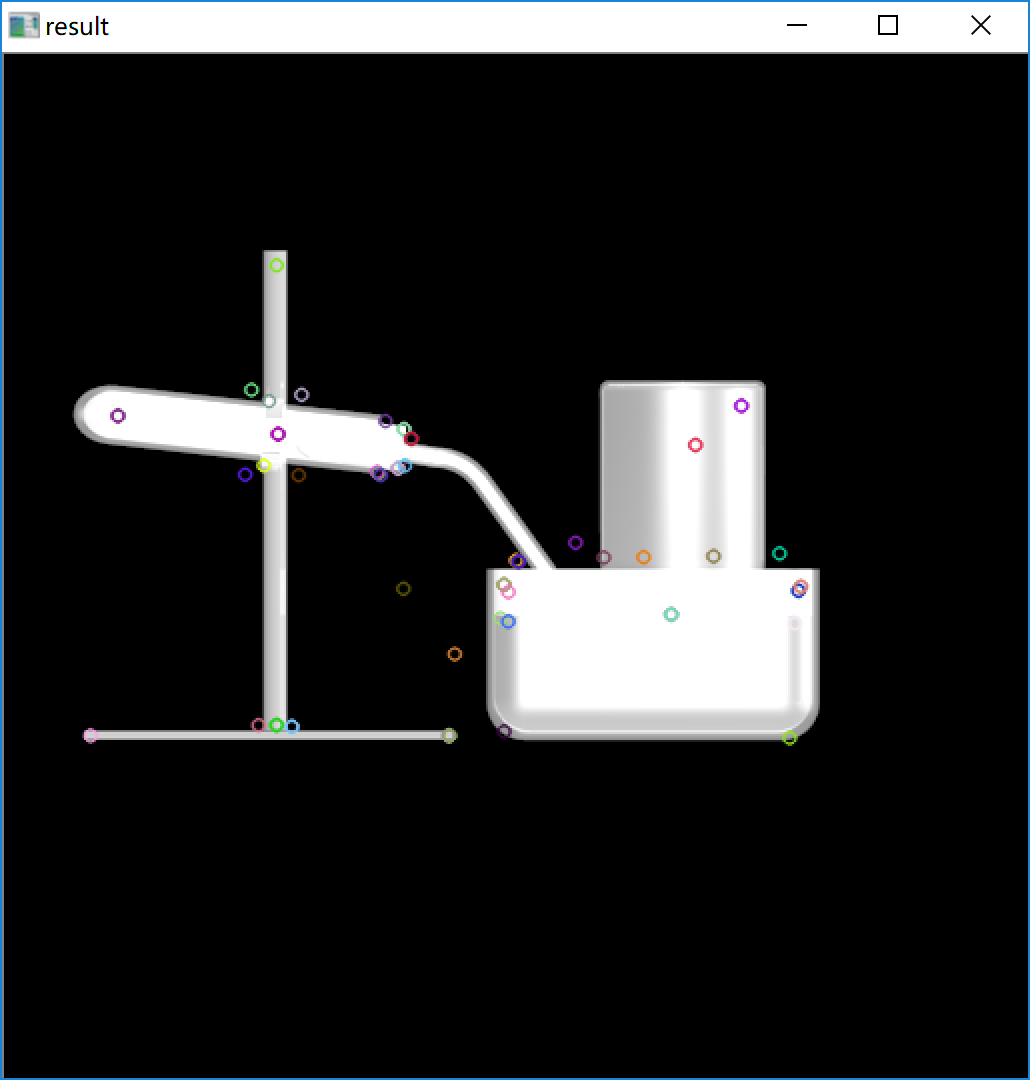
\includegraphics[width=0.8\textwidth]{images/SIFT-origin.png}
    \caption{使用SIFT检测原图特征}\label{fig:digit}
    \end{figure} 
    
    \qquad 检测效果受到了模型的高光影响,甚至在背景中也出现了key point。为了去除这些干扰信息,我们又使用SIFT对轮廓图进行了特征提取。
    
    \begin{figure}[h]
    \centering
    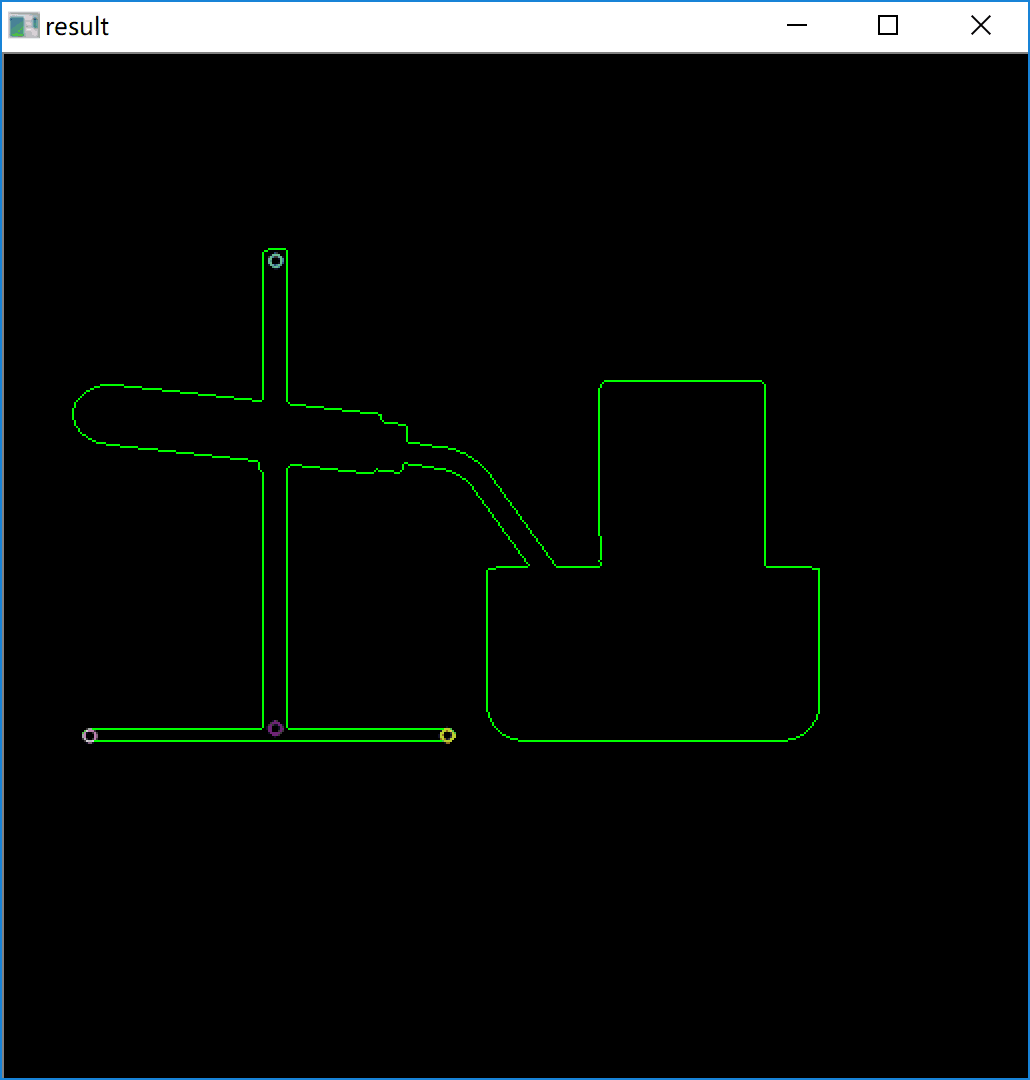
\includegraphics[width=0.8\textwidth]{images/SIFT-countour.png}
    \caption{使用SIFT检测轮廓图特征}\label{fig:digit}
    \end{figure} 
    
    \qquad 然而,使用轮廓图作为检测的原图又会导致key point减少的问题。在示例轮廓图中,整个右部都没有特征点。考虑到SIFT算子相对来说实时性还不够高、特征点较少、对边缘光滑的目标无法准确提取特征点等缺点,我们在这两次实验后放弃了SIFT算子提取轮廓的方法。
    
    \qquad 这之后我们又尝试了傅里叶描述符 (Fourier Descriptor) 。
    
    \qquad 傅里叶描述符(Fourier Descriptor)将物体的形状看做是一条封闭的曲线,称为边界曲线。
    把曲线上的点`(x,y)`表示为复数形式`(x+yi)`,就可以把边界曲线看作描述点变化的周期函数,这个函数用傅里叶级数展开,将得到一系列复数形式的系数,它们共同描述了边界的形状。
    
    使用傅里叶描述符来提取特征的过程:
    \begin{enumerate}
        \item 得到原始傅里叶描述符
        
        \qquad 首先提取图片的轮廓曲线,将曲线中的点坐标表示为 $$ x + y i $$的形式,对复数点集进行傅里叶展开,这样就得到了原始的傅里叶描述符
        
        \item 降低描述符degree
        
        \qquad 由于轮廓曲线中的点比较密集,所以得到的描述符的degree也比较高,所以可以对描述符进行重建,降低degree,方便减少存储的空间,也利于特征匹配。
        
        \item 对提取的描述符进行逆变换
        
    \begin{figure}[htb]
    \centering
    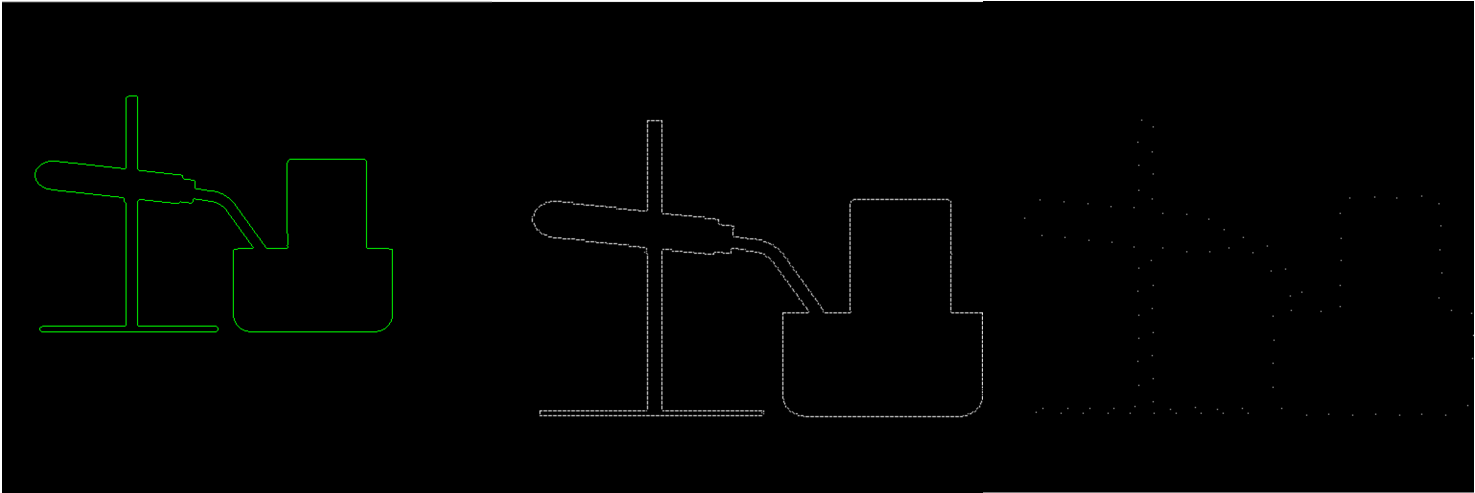
\includegraphics[width=1\textwidth]{images/Fourier.png}
    \caption{原始轮廓 / 高度数描述子逆变换轮廓 / 低度数描述子逆变换轮廓}\label{fig:digit}
    \end{figure} 
        
        \qquad 使用傅里叶描述符提取效果良好,描述子也可以很方便的存储为npy数组文件格式,因此我们决定使用傅里叶轮廓描述符进行特征提取。
        
    \end{enumerate}
        
    \end{enumerate}
    
    \item 视图特征匹配
    
    我们尝试了两种特征匹配方法:
    
    \begin{enumerate}
        \item 向量机
        
        \qquad 把匹配问题看作一个分类问题,使用支持向量机(Support Vector Machine, SVM)对输入的数据分类到不同的模型。
        
        \item K-最近邻
        
        \qquad 使用K最近邻(kNN,k-NearestNeighbor)分类算法,使用最近的K个邻居的类别作为输入的类别。
        
    \end{enumerate}
    
    \qquad 由于目前没有足够的训练数据,我们对20个模型的正视图提取了描述符,然后对描述符增加高斯噪声来生成训练和测试数据。
    
    \qquad 设置训练集和测试集的大小为2000(每个模型有100个样本),在不同描述符degree下分类的粗略结果如图表所示:
    
    \begin{figure}[htb]
    \centering
    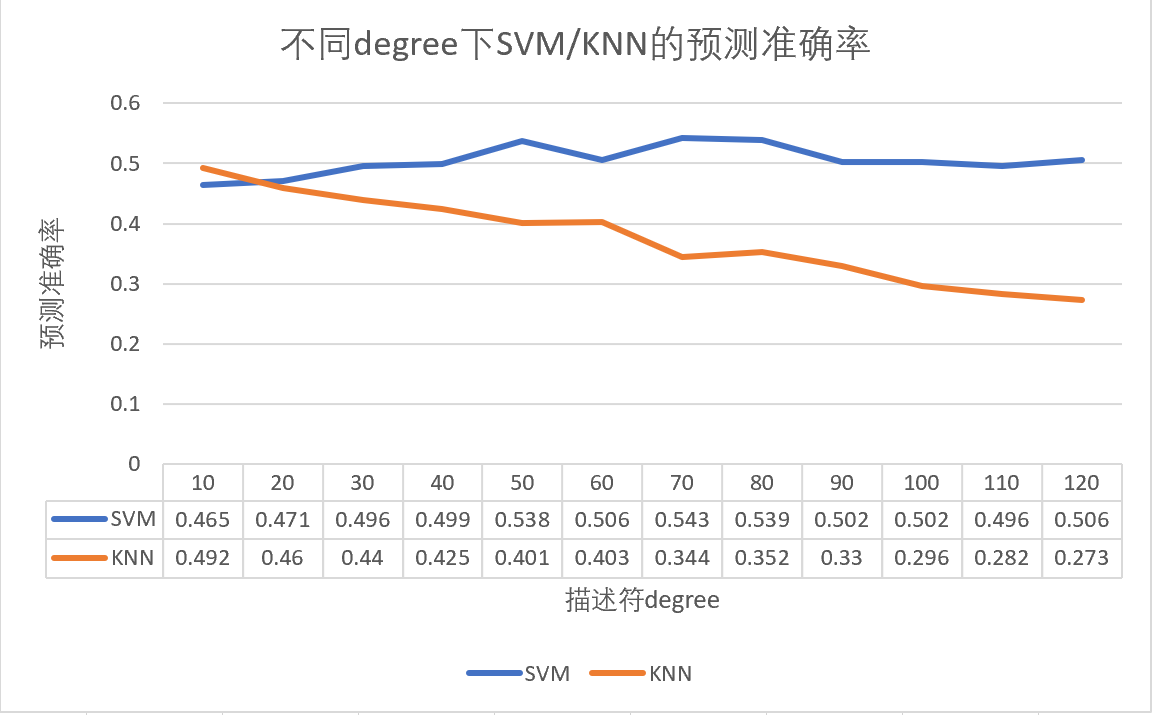
\includegraphics[width=1\textwidth]{images/predict.png}
    \caption{不同Degree下SVM/KNN的预测准确率}\label{fig:digit}
    \end{figure} 
    
    对此测试结果,我们分析如下:
    
\begin{itemize}
    \item  degree对分类准确度有较大影响,后续需要调整合适的训练参数
    \item 目前的准确率都比较低,但是考虑到随机样本的不真实性,我们打算后续使用手绘简笔画进行进一步的测试和调整
\end{itemize}

\end{enumerate}

\clearpage
\newpage

\section{工作内容}

\subsection{已完成工作内容}
\begin{enumerate}
    \item VR模块
    
    \begin{enumerate}
    \item 绘画模块
    \item 导出绘画信息
    \item 导入模型
    \end{enumerate}
    
    \item 模型检索模块
    
    \begin{enumerate}
    \item 模型三视图渲染
    \item 三视图特征提取
    \item 特征匹配
    \end{enumerate}

\end{enumerate}

\subsection{分工完成情况}
\begin{tabular}{cccc}
\toprule  %添加表格头部粗线
姓名& 学号& 分工& 完成情况\\
\midrule  %添加表格中横线
罗宇辰& 516030910101& 模型检索模块& 模型三视图渲染,三视图特征提取,特征匹配\\
陈志扬& 516030910347& VR模块& VR绘图,导出模型\\
陈\quad 诺& 516030910199& 模型检索模块& 资料查找,三视图特征提取,文档及PPT 
\toprule 
\bottomrule %添加表格底部粗线
\end{tabular}

\subsection{后续工作内容}

\begin{enumerate}
    \item VR模块
    
    \begin{enumerate}
    \item 提高画笔在黑板上绘画的真实感
    \item 提供板擦
    \item 提供多种颜色和粗细的画笔
    \end{enumerate}
    
    \item 模型检索模块
    
    \begin{enumerate}
        \item 提高检索准确率
        \item 针对简笔画输入优化特征提取模块
        \item 提供快速扩充模型库的方法
    \end{enumerate}
    
\end{enumerate}

\end{document}
